\documentclass[12pt]{article}
\usepackage{amsmath,amssymb,graphicx,paralist,setspace,amsthm,pdflscape,fancyhdr,fullpage,rotating,tikz,xcolor,float,varwidth,comment,multirow,array,makecell}
\usepackage{sectsty}
\sectionfont{\centering\large}
\subsectionfont{\centering\normalsize}
\usepackage{subfigure}
\usepackage{longtable}
\usepackage[]{har2nat}
\setcitestyle{aysep={}}
\setcitestyle{notesep={, }}
\usepackage{mathtools}
\usepackage{url}
\usepackage{placeins,float}

\makeatletter
\g@addto@macro{\UrlBreaks}{\UrlOrds}
\makeatother

\usepackage{appendix}
\newtheorem{hyp}{Hypothesis}
\usepackage[space]{grffile}
\usepackage[urlcolor=blue,citecolor=blue,linkcolor=blue,linktocpage=true,backref=true]{hyperref}
\usepackage{setspace} % load setspace before footmisc
%\usepackage{footmisc}
%\renewcommand{\footnotelayout}{\doublespacing}
%\setlength{\footnotesep}{\baselineskip}
\hypersetup{
	colorlinks=true,
	urlcolor=blue
}
\usepackage[space]{grffile}
\bibliographystyle{apsr}
\usepackage{siunitx}
\sisetup{
	table-parse-only = true,
	tight-spacing           = true,
	input-open-uncertainty  = ,
	input-close-uncertainty = ,
	round-mode              = none,
	round-precision         = 3,
	table-space-text-pre    = (,
	table-figures-integer = 3,
	table-figures-decimal = 3,
	table-figures-exponent = 2,
	table-align-text-pre  = false,
	table-align-exponent = true,
	table-space-text-post   = )\Star,
}
\protected\def\Star{$\text{*}$}
\newcommand\Mycomb[2][^n]{\prescript{#1\mkern-0.5mu}{}C_{#2}}
\newcommand{\possessivecite}[1]{\citeauthor{#1}'s \citeyear{#1}}
%\raggedright
\makeatletter
\newcounter{subhyp} 
\let\savedc@hyp\c@hyp
\newenvironment{subhyp}
{%
	\setcounter{subhyp}{0}%
	\stepcounter{hyp}%
	\edef\saved@hyp{\thehyp}% Save the current value of hyp
	\let\c@hyp\c@subhyp     % Now hyp is subhyp
	\renewcommand{\thehyp}{\saved@hyp\alph{hyp}}%
}
{}
\newcommand{\normhyp}{%
	\let\c@hyp\savedc@hyp % revert to the old one
	\renewcommand\thehyp{\arabic{hyp}}%
} 
\makeatother
\begin{document}



\author{Michael A. Allen \\ Department of Political Science \\ Boise State University \and Brian D. Blankenship \\Department of Political Science\\University of Miami \and Michael E. Flynn \\ Department of Political Science \\ Kansas State University \and Renanah Miles Joyce \\ Department of Political Science \\ Brandeis University \and Carla Mart\'{i}nez Machain \\ Department of Political Science \\ University at Buffalo}
\title{Great Power Competition for Military Access in Kenya \footnote{We would like to thank...}}

\date{\vspace{2em}\today \vspace{1em}}

\maketitle

\thispagestyle{empty}

\clearpage

\begin{abstract}
\noindent 

This project highlights unique features of the China-U.S. relationship and presents new hypotheses on the interaction between democratic and autocratic powers in their competition for international influence.
\end{abstract}




	\vfill
	
	\thispagestyle{empty}
	
	
	\newpage
\setcounter{page}{1}

\doublespacing
	The opening of China's People's Liberation Army base in Djibouti in 2017, its first permanent military installation abroad, was a key moment for Chinese foreign policy. It launched discussion and speculation about whether China's growth in power and influence would lead it to seek a foreign military base network to rival that of the United States \cite{vertin2020}. Yet, in the seven years since, we have not seen as strong of an effort from China to continue to build military installations abroad. Ream Naval Base in Cambodia was renovated with Chinese funds, and Chinese military vessels have docked there since 2023 and maintained access \cite{gan2023}. Beyond that, while there has been talk of China having an interest in locations such as the UAE or the Solomon Islands, there has yet to be a sharp increase in Chinese military installations.

Does this mean that China does not have global military ambitions? Is it scaling back on its quest for global political influence? We argue that this is not the case but rather that China is following a pattern of influence that is different from that of the United States and other former colonial powers such as Britain and France. By forcing China into the U.S. model of foreign military influence and expecting it to set up military bases under the American model, we are missing observations and lacking a fuller understanding of Chinese foreign military policy. 

The ability to project military power abroad is a central means by which states exert influence in international politics, allowing them to defeat adversaries and reassure allies across large distances \cite{levy2010,markowitz2013,blankenship2022}. To project power, states need access to other countries' territory, often in foreign military bases, which allow states to control territory, forward deploy personnel, and resupply their forces \cite{Harkavy1989,posen2003}. Basing access, however, is often precarious. In the current international system, states typically rely on the consent of sovereign host states to build and maintain their foreign military presence. This strategy contrasts with earlier periods when states secured bases through force, coercion, and formal empire \cite{schmidt2020}. Because host states can grant or deny access, they are subject to pressure as great power rivals like the United States and China increasingly compete for military access and influence worldwide.

The systematic study of overseas military basing and how it affects and is affected by host populations is still new. While military basing is a centuries-old practice, methods of securing military access have evolved. Traditionally, the ability to deploy troops in other states' territory primarily arose from conquest and colonialism. After World War II and the period of decolonization, alliances and regime change provided a path for the United States and the Soviet Union to have long-term military access to (or control over) others' territories. While the collapse of the Soviet Union led to the withdrawal of most Russian bases, the United States expanded its network to cover most of the globe.

In several ways, the emerging era of great power basing is distinctive from either the Cold War or post-Cold War periods. First, unlike the post-Cold War period, the United States faces geopolitical competition from near-peer great powers like China. As a result, the challenges to U.S. bases no longer stem solely from internal forces—concerns among the population about crime, pollution, and infringements on sovereignty—but also have an essential external component\cite{allen2023}.

Second, unlike the Cold War, China's challenge to U.S. bases is often more indirect and asymmetric than that of the Soviet Union. The U.S. and the Soviet Union competed for bases directly but rarely had bases in the same countries \cite{Nieman2020}. China, by contrast, has pursued a lighter-footprint military presence model and has often sought access and influence in countries that could or already do host a U.S. base. For example, China placed its permanent military base in a country that already hosted Africa's largest U.S. base. Similarly, much of China's effort has focused on establishing military access to other states' existing military or commercial installations, such as dual-use commercial ports \cite{kardon2022}. China has thus followed a different power projection model that better fits with a strategy of avoiding confrontation and building political, economic, and military influence \cite{Doshi2021}. The aforementioned example of gaining access to Cambodia's Ream Naval base fits this model \cite{gan2023}.


In this project, we take the case of Kenya, which allows us to observe the American and Chinese models for military access and influence side by side. The U.S. maintains a military presence at the Manda Bay Airfield in southeastern Kenya, which the Kenyan Defense Forces operate, but also hosts a U.S. military presence of approximately 50 troops \cite{allen2022}. China's influence on Kenya is mainly expressed through large amounts of Chinese foreign direct investment on infrastructure through the Belt and Road initiative and sovereign debt incurred from China \cite{lesutis2021}. Yet along with this economic influence, China has also gained military access, albeit in a much smaller footprint form than that of the United States: A 2023 U.S. Department of Defense report notes that China's People's Liberation Army Strategic Support Force ``operates tracking, telemetry, and command stations'' in Kenya \cite{DOD2023}. 

%The United States and China have increasingly sought to influence African nations through economic, military, and diplomatic channels to gain military access to countries. Such projects include China's Belt-and-Road Initiative, the United States constructing limited footprint bases like the drone base in Niger, and both countries maintaining a military presence in Djibouti. As part of an exploratory analysis to see how influence campaigns in Africa affect the perceptions of host-state civilians, we deployed a survey in Kenya. Kenya represents a case where the country has stronger military ties to the United States while also experiencing active influence efforts by China. Given that military access increasingly requires the consent of the public and not just elites, the perception of civilian actors can influence Kenya's military alignment in the long run. 


A recent U.S. Institute of Peace (USIP) report notes that many African states are becoming wary of military presences within their territories. Though a military presence or base can be profitable for leaders (see Djibouti as an extreme example), ``military bases can also be a political liability for African governments that host them'' \cite{usip2024}. This opinion is not a new sentiment. As noted in the report, a 2016 African Union report ``noted with deep concern the existence of foreign military bases and establishment of new ones in some African countries'' and ``stressed the need for Member States to be always circumspect whenever they enter into agreements that would lead to the establishment of foreign military bases in their countries'' \cite{AU2016}.Thus, if China and the U.S. want to expand or maintain their military presence in Africa, they will have to convince not only elites but also members of the population to accept this presence, whatever shape it may take. This will be particularly true in democratic or partly democratic states such as Kenya. 

This project thus compares the two influence models of the United States and China by studying Kenyans' perceptions of the U.S. and China generally and their views on Chinese and U.S. military presences in their country. Following previous work, we expect that both personal interactions with individuals from a major power, as well as the cultural influence that is created from that major power's presence or investment in the country (be it military or not) will lead to more positive views of the major power, as well as greater acceptance of granting the major power access to the country. Regarding the effectiveness of the Chinese vs the American approach, we remain agnostic and treat the study as exploratory in comparing Kenyan views of both countries. To test these questions we deployed a survey to Kenya in the summer of 2023 to assess the cross-competing effects of influence campaigns by the United States and China. Despite Kenya's ties to the United States, Chinese influence campaigns in the region are prominent and effective. 







	\section*{Theory}

Since the end of the Cold War the United States has maintained an unrivaled network of global military bases. This access to foreign military territories has allowed the United States to maintain a global sphere of influence, assure allies, and threaten intervention in response to emerging threats. However, even a global basing network does not provide unfettered access. An example of the United States being constrained by its basing hosts occurred in the lead-up to the U.S. invasion of Iraq in 2003. The United States, which maintained between 2,000–3,000 troops in Turkey, requesting the use of Turkey as a launching pad for its invasion. Unexpectedly, the Turkish parliament refused the U.S. request. The unexpected negative vote was attribute to many factors, including disunity within the ruling party and a Turkish attempt to gain more concessions from the United States, as well as Turkish public opinion that was overwhelmingly against the war \cite{otterman2005}. 

As this example illustrates, access is an ongoing political and bargaining process that requires consent from the granting state. Moreover, this bargaining process often encounters internal challenges from domestic audiences within a host country who oppose the foreign military presence, or the actions that may be launched from the host territory, as was the case in Turkey and as has been the case in German protests against U.S. drones being operated from Ramstein Air Base. Internal challenges can be ideologically rooted, such as opposition to infringement upon host sovereignty or pacifist sentiment, or may derive from the negative effects that bases impose on their environments, including noise, environmental pollution, traffic congestion, and crime committed by the basing power's service members \cite{kim2023}.

To overcome these potential objections, basing countries use different policy tools to win both elite and popular support for a military presence. These include using financial incentives to curry favor---such as building infrastructure for the host population and hiring local labor—as well as taking steps to ensure that the host population has positive social interactions with military personnel \cite{allen2020,blankenship2020,allen2023}. As reported by the Washington Post in April 2023, the U.S. Department of Defense believes that ``the PLA likely will use tailored approaches to address local concerns as it seeks to improve relations with amenable countries and advance its overseas basing goals'' \cite{hudson2023}. The U.S. State Department similarly noted in 2018 that ``the United States has created a strong Djiboutian constituency that favors our military presence, owing to increased local hiring and contracting with Djiboutian companies at Camp Lemonnier'' \cite{state2018}. 

Despite the importance of these tools in cultivating host support and the centrality of host support to bargaining over access, both support and its drivers remain understudied. This is particularly true in the present era of competition between the United States and China. Moreover, much of China's challenge to U.S. bases is economic rather than directly military in nature. China has emerged as a massive source of global lending and foreign investment, particularly since the announcement of the Belt and Road Initiative in 2013, and many recipients of Chinese investment are U.S. base hosts, while the United States is also a major investor and also uses economic power to create security influence. This type of economic influence from a rival power poses at least two challenges to a competitors' basing efforts. First, that rival can actively seek to use its economic incentives to convince policymakers or the public within a host state to block access to a rival power seeking to build or expand a new military base \cite{joyce2023}. For example, the United States has actively pressured its ally, the United Arab Emirates, to scrap a plan to allow for the installation of a Chinese military facility near Abu Dhabi \cite{hudson2023}. Second, the rival's economic engagement can crowd out the incentives the basing country offers, making the incentives seem less attractive by comparison \cite{joyce2023}.
%[Probably need to add more here. Maybe something about economic influence translating to cultural influence, which is going to be what we argue in the hypotheses]

\subsection*{Economic and Cultural Influence}
%[RJ: Nye and others generally include economic threats and payments under hard rather than soft power. Probably either modify this framing to make it about hard and soft power (e.g., Nye's "smart power", or explain how/why we are treating economic incentives as soft power here]

Soft power as a force for influence in international relations gained prominence as the Cold War was dying down \cite{nye1990}. The idea that norms, culture, and ideas can influence international relations is certainly older than the coining of the term soft power. However, with the transition from bipolarity to hegemony, international relations scholars found new interest in the concept of soft power. 

Soft power can work through a few different mechanisms. Notably, it is less directly coercive than hard power in that the pulls of economics, ideas, and culture become a gravitational force for other countries and their populations. Different actors may see another country's success and wish to model their institutions after that country to emulate their successful model. Alternatively, people may adopt the ideas and beliefs of the soft power-producing country and see the world through similar eyes. Soft power works well when actors agree upon their vision for the world and the paths to achieve those goals.

The nature of soft power and the instruments that contribute to it evolve with culture and economics. Much as globalization has reshaped communication, trade, and culture, globalization is an ongoing process that also alter the tools of soft power. While music became a catalyst for soft power during the Cold War and remains a vital element in expressing cultural values, other venues continue to emerge and establish themselves \cite{nye2004}. Likewise, sports and movies are classic conduits of soft power\cite{sari2012,grix2014}. Social media created a new wave of ways in which individuals and states can access individuals directly, and the occupation of influencer arose in the 2000s.\footnote{The role of influencer is certianly historic and predates the modern incarnation. For example, movie celebrities and the rise of the fashion industry was a incarnation of the influencer role.} Scholars have noted how influencers within a country can promote the messages of foreign governments through social media channels \cite{vibber2021}. 

The role of influencing people through online media is not unique to just personalities, but may concern the platform those personalities occupy. Initially, much of the dominant social media came from Western countries through Myspace, Facebook, YouTube, Reddit, and Instagram, but Chinese companies have competed in that space with Weibo and TikTok. In recent years, there has been growing concern about which countries control which social media platforms, what those companies and governments do with the data from the platform, and how that can influence society, culture, and politics.  

The United States, Russia, and China have engaged in extensive campaigns of economic and cultural influence throughout the globe. Influence sources for these competing actors exist with official policy, such as aid and the Belt-and-Road initiative, social media, and interpersonal contact between foreign nationals and civilians. Soft power can stem from Chinese and American nationals who are in other countries for personal, business, or official state capacities. Deployed military members overseas are a source of soft power that builds support for the missions they engage in through their official activities and everyday activities as private individuals \cite{atkinson2014,allen2023}. Patronage of local establishments, raising a family in a host community, or attending local events can normalize and encourage support of a foreign military presence. 

In all of these ways, soft power is vital instrument in securing military access and building support from the ground up for a nation becoming aligned with another government.


\subsection*{The Politics of Influence and Military Access} 

Early scholarship on foreign military basing focused on understanding how great powers acquire, use, and compete for bases. Perhaps most notably, Robert Harkavy's \citeyear{Harkavy1982,Harkavy1989,Harrison2000} work offered sweeping accounts of great power bases over eight centuries, with particular emphasis on how the United States and Soviet Union attempted to acquire bases and deny them to each other using various economic, political, and military tools. Other scholars focus primarily on the United States, attempting to chronicle the scope and purpose of the vast U.S. basing network during and after the Cold War \cite{vine2015,moore2016,sandars2000}. This body of scholarship, however, is largely descriptive and almost exclusively focused on government-to-government interactions.

More recently, scholars have opened the black box of basing relationships to explore how domestic politics in host countries can shape the political viability of overseas bases and how basing countries, in turn, can adapt. \citeasnoun{calder2008}, \citeasnoun{Cooley2008}, and \citeasnoun{yeo2011} all shed light on how domestic anti-base movements can pressure host governments to evict foreign militaries, particularly during periods of democratic transition. Building on this work, \citeasnoun{allen2023} explore the micro-foundations of domestic support for foreign bases using surveys across fourteen countries, with findings suggesting that positive economic and social interactions between U.S. personnel and the host population can build support for the U.S. military presence.

These two strains of literature have mainly remained separate, leaving a gap in our understanding of how great power competition can shape the foundations of domestic support for hosting foreign bases. This competition can be directly military, as in the case of U.S.-Soviet competition for bases during the Cold War \cite{Nieman2020,Harkavy1982}. It can also be broader, with rivals seeking political, economic, and cultural influence across the same countries. For example, China has primarily sought influence with economic tools, perhaps most notably through its Belt and Road Initiative, which has financed some \$500 billion in infrastructure globally since 2008. China has relied on access to infrastructure like ports through the ownership rights of state-owned enterprises to project power, as in Cambodia \cite{kardon2022,kardon2022pier}. Additionally, China acquired the rights to its first foreign military base in Djibouti in 2015, and since then has sought base rights in countries across Asia, Africa, and even the Americas \cite{hudson2023,strobel2023}. Leaks of Department of Defense documents, reported by the Washington Post in April 2023, revealed U.S. military estimates that ''the PLA seeks to establish at least 5 overseas bases and 10 logistic support sites by 2030 to fulfill Beijing's national security objectives, including protecting its economic interests abroad''\cite{hudson2023}. Even where China does not seek bases, its economic footprint poses problems for the United States, as China can use its influence and economic leverage to deny U.S. access. In Kenya, for example, U.S. officials have indicated their alarm at the country's willingness to hire a Chinese construction firm to complete upgrades to a joint Kenya-U.S. counter-terrorism base unless the United States pays for the upgrades itself, fearing that the Kenyans could leverage geopolitical ties with China for economic gain \cite{philips2023}.

This project attempts to fill this gap by exploring how major powers can derive influence in foreign countries through military, social, economic, and cultural contact with local populations. It argues that whether this is an intentional strategy or not, this influence can facilitate the acquiring and maintenance of military access to these states. Importantly, we study this question taking into account the possibility that more than one major power may be competing for access to these third-party states. One major power's influence campaigns may limit its rival's ability to gain military access to a third-party state. We will thus explore how major powers' influence attempts can be undermined (or not) by those of rival major powers. In doing so, we will shed light on additional mechanisms through which great power competition can shape foreign military deployments beyond government-to-government interactions. 

From the military basing side, much of the literature has focused on great power competition in the context of U.S.-Soviet Cold War relations. The host countries studied have generally been in regions like Europe and East Asia. The literature focused on major powers' quest for influence in Africa has tended to study it in terms of influence by former colonial powers, or with a greater focus on purely economic investment and aid. Yet there is a lack of work on the competition for military access to African states, particularly in democratic ones such as Kenya. In the current environment, competition for bases and military access occurs in a world characterized by strong norms of sovereignty, in which access must be granted consensually and in which many hosts are either democratic or could democratize \cite{Cooley2008,schmidt2020}. Therefore, understanding the mechanisms that govern the consent of domestic populations toward foreign military basing and deployments is crucial for comprehending the conditions under which great powers can project power abroad. 

What instruments are likely to build consent among domestic populations? A well-studied source of power in international relations is the ability to change other actors' incentives to make it rational for them to comply with an actor's preferences \cite{dahl1961}. Aside from the threat or use of force—which has over time become a less common means of securing foreign bases—states can use positive inducements to structure other actors' incentives \cite{schmidt2020,Lake1996}. Indeed, the literature suggests that states often use tools of economic statecraft like foreign aid to buy foreign policy influence and secure access to bases \cite{carter2015,alexander2019,blankenship2020,joyce2023}. However, there is some evidence that this effect may vary across states. A recent study of U.S. and Chinese aid to 38 different African countries found a link between U.S. aid and positive views of the United States. However, Chinese aid did not affect public support or actively reduce it \cite{blair2022}. This divergence suggests that major powers who compete for public approval using similar tools may not achieve similar effects, and highlights the need for research to study how such interventions may uniquely affect civilians in host countries.

Beyond structuring other actors' incentives, states can also attempt to elicit cooperation through soft power. Overseas military deployments can be a source of soft power \cite{atkinson2014}. First, the most obvious way military deployments can encourage soft power is through humanitarian missions where service members assist with health care or disaster relief. These acts build support for the basing country as it is clear that the assistance comes from the base power \cite{flynn2019}. Second, service members integrated into overseas communities can build soft power, although this is harder to observe. Routine daily behavior by service members on and off base creates potential points of interaction that can build support for a basing country's mission in a host country. Research finds that interactions with service members can reduce stereotypes, build goodwill, and humanize a deployed force such that contact alone can produce positive assessments of a foreign-deployed army \cite{allen2023}. States with an active, non-isolated presence can actively build support for their presence with local populations. As such, we expect interactions with U.S. and Chinese individuals will garner support for each country and its military within Kenya. This creates our first set of hypotheses:

\begin{subhyp}
	
	\begin{hyp}
		Interpersonal contact with U.S. individuals correlates with more positive views of the United States.
	\end{hyp}
	
	\begin{hyp}
		Interpersonal contact with Chinese individuals correlates with more positive views of China.
	\end{hyp}
	
\end{subhyp}

\begin{subhyp}
	
	\begin{hyp}
		Interpersonal contact with U.S. individuals correlates with more support for hosting the U.S. military.
	\end{hyp}
	
	\begin{hyp}
		Interpersonal contact with Chinese individuals correlates with more support for hosting the Chinese military.
	\end{hyp}
	
\end{subhyp}

Moreover, given our discussion about the role of cultural influence through sporting events, entertainment, and other advertising vehicles, we expect sources of cultural influence to correlate wit positive views of each country and its military in our second set of hypotheses.


\begin{subhyp}
	
	\begin{hyp}
		More exposure to U.S. cultural influence correlates with more positive views of the United States.
	\end{hyp}
	
	\begin{hyp}
		More exposure to Chinese cultural influence correlates with more positive views of China.
	\end{hyp}
	
\end{subhyp}

\begin{subhyp}
	
	\begin{hyp}
		More exposure to U.S. cultural influence correlates with more support for hosting the U.S. military.
	\end{hyp}
	
	\begin{hyp}
		More exposure to Chinese cultural influence correlates with more support for hosting the Chinese military.
	\end{hyp}
	
\end{subhyp}

Additionally, existing scholarship indicates rival providers can undermine states' influence attempts. The literature on foreign aid and economic statecraft, for example, suggests that states and international organizations like the World Bank are less able to make their assistance conditional on policy concessions when recipients have alternative sources of aid and financing \cite{dunning2004,bdm2016,woods2008,kastner2021,watkins2022}. %Do we want hypotheses for these?


However, the literature leaves gaps in our understanding of great power inducements and influence. For one, tools of influence—such as foreign aid, military contact, and military training—are typically studied independently rather than comparatively. Research on influence and policy concessions also tends to ignore military bases and focuses on government-to-government interactions rather than government-to-public interactions, while work on influence and public opinion tends not to focus on public support for policy concessions and tends to ignore the role of foreign competition. Indeed, while the U.S. Department of Defense worries that the PRC targets countries for future military installations, we know little about the ``host nation receptivity'' to these intentions \cite{hudson2023}. %This project fills these gaps by offering evidence on the relative importance of soft power coming from different instruments (military versus non-military) and different actors (the United States versus China) under conditions of competition.

Thus, given existing literature on the role of international competition in undermining states' influence attempts \cite{joyce2023}, we might expect that exposure to contact with U.S. and Chinese individuals, economic footprints, and culture will negatively correlate with support for hosting the other's military presence.

\begin{subhyp}
	
	\begin{hyp}
		More exposure to U.S. individuals and influence correlates with less support for hosting the Chinese military.
	\end{hyp}
	
	\begin{hyp}
		More exposure to Chinese individuals and influence correlates with less support for hosting the U.S. military.
	\end{hyp}
	
\end{subhyp}


As we describe in more detail below, we test these hypotheses using a survey instrument in which we ask respondents about their contact with U.S. and Chinese citizens and about their exposure to the culture of one or both of these major powers. Respondents are then asked about their level of support for those countries' bases.








	\section*{Research Design}

To test our hypotheses, in September 2023, we developed and deployed a survey instrument in Kenya. We deployed the survey in English and Swahili to 1,023 Kenyans via SMS (text message) using the survey firm GeoPoll, which has extensive experience in Kenya, to implement the survey. Respondents were over 18 years of age and recruited by Geopoll using a database of mobile phone numbers across Kenya.\footnote{While most people reported their primary language being Swahili, most respondents opted to take the survey in English} The survey was nationally representative on age and gender. GeoPoll incentivized respondents with airtime credit (about 0.50 USD, in local currency) to respond to the survey, which took approximately 15 minutes to complete, on average.\footnote{0.50 USD translated to 69 Kenyan Shillings at the time of the survey. This would roughly cost a 12 oz bottle of Coke or Pepsi. This amount met the minimum threshold necessary to motivate participation based on GeoPoll's experience operating in Kenya.} Although this limited the sample to only people who own mobile phones, mobile use is widespread enough in Kenya that this did not limit our sample in a significant way. We collected the full sample over six days.  

In the survey, we intentionally oversampled respondents from Mombasa County (50\% of respondents), as this is where the United States maintains its military presence. The rest of the sample is nationally representative of the Administrative 1 (ADM1) location. Oversampling Mombasa County increases the probability of respondents having had contact with the U.S. military, thus allowing us to assess whether contact with service members influenced views of the United States or its military presence. Though it would not give us an accurate representation of how likely an individual would be to have contact with a member of the U.S. military, in general, we note that our hypotheses are not about the frequency of contact but about the effect that contact can have on views of major power military access. 

The survey contained 28 questions. It included demographic questions of age, gender, language spoken at home, household income, and the county in which the respondent lives. These questions allow us to sample representatively and control for demographic factors that may influence views on foreign military access.

\subsection*{Dependent variable} 

Our hypotheses focus on two dependent variables: General views of a major power (either China or the United States) and support for hosting a major power's (China or the U.S.) military in Kenya. 

To measure the first dependent variable (general positive or negative views on a major power), the survey asked questions about the perceived influence of the major powers on Kenya (``How much economic and political influence does China/the United States have on Kenya?''), with answer options being ``A lot'', ``Some,'' ``A little,'' ``None,'' and ``Don’t know / haven’t heard enough.'' We also asked whether that major power's influence was positive or negative, with response options being ``Very negative,'' ``Somewhat negative,'' ``Neither positive nor negative,'' ``Somewhat positive,'' and ``Don't know/no opinion.'' We also asked respondents about which country they thought ``should be a model for [Kenya's] future development''. Besides China and the United States, we also 
included Britain (as a former colonial power), other African states, India, and options for ``Other'' and ``None of these,'' not to force respondents to choose only between the United States and China.

To measure the second dependent variable, the level of support for a major power's military presence in Kenya, we ask respondents ``In general, what is your view toward the United States/China having a military presence in Kenya?'' The options again ranged from ``Very Negative'' to ``Very Positive,'' with the option to respond ``Don’t know / Decline to answer.''\footnote{We note that before asking about the respondents' views towards the foreign military presence, we first asked them if, to their knowledge, the United States/China has a military presence in Kenya.}  

\subsection*{Independent variables} 

Our hypotheses also focus on two key independent variables (both of which we expect to influence both views of the major powers and support for their military presences). The first is interpersonal contact, and the second is cultural influence. They are both measures of soft power, but one is a direct social interaction, whereas the other measures the exposure of individuals to media such as film, TV programs, sporting event broadcasts, social media, and foreign education destinations. 

For contact, we first asked respondents if they had had ``face-to-face contact with a citizen of the United States/China in Kenya?'' If they responded yes to this question, we then asked them several follow-up questions about the nature of that contact. We first asked them about the frequency of contact, ranging from ``Daily'' to ``Once.'' The next question asked about the type of contact had, giving them a list of options for forms of contact (ranging from ``a brief everyday interaction'' to ``Dated/were romantically involved with'' a person from the major power of interest).\footnote{See appendix for the full list of response options} Respondents were allowed to select all options that applied to them and an ``Other'' option. Finally, we asked whether any of that contact was with ``a member of the U.S./Chinese military'', to determine whether any direct contact was happening between deployed military personnel and locals in Kenya. In the survey we first asked respondents this set of questions about the United States and China.

To ask respondents about their exposure to cultural influence, we asked the about the country of origin of ``the last film you watched in a theater,'' ``the last television program you watched,'' and ``the last athletic event you watched.'' In addition, we asked them about the social media app that they used most often, to gauge the popularity of U.S.-owned apps such as Meta, Whatsapp, or Instagram or Chinese-owned ones such as TikTok. Finally, we asked about any family members who had gone abroad to study, and which country was the most common destination.\footnote{Besides China and the United States, the other options given were ``Britain,'' ``Ethiopia,'' ``South Africa,'' and ``India,'' as well options for ``Other'' and ``None.''}

\subsection*{Control variables} 

In addition to our independent variables, we include a series of demographic questions that could affect perceptions of China and/or the United States and the likelihood of having contact with foreign citizens and being exposed to foreign cultures \cite{clarke2005}. We asked about income levels, as wealthier individuals may have more cosmopolitan attitudes about foreign states, have traveled more, and are more receptive to foreign influences. We also included a variable for the highest level of schooling completed, again with an expectation that education may correlate positively with openness to foreign ideas and individuals.

In addition, because past work has found that women may be less receptive to militaristic policies than men, we also take into account the respondent's sex \cite{allen2020,allen2023}.\footnote{At the advice of the survey firm's country expert who noted this issue could be culturally sensitive, we did not include a ``non-binary'' option in this question, instead asking about sex (rather than gender) and included a ``Prefer not to say'' option.} Finally, because we expect that young people may both be more likely to hold liberal, anti-militaristic policies but also be more likely to be exposed to foreign media and influences, we asked about the respondents' age. 



	\section*{Results}


The preliminary results point to some interesting dynamics. 40\% of respondents view China as having both ``A lot'' of influence and ``Somewhat positive'' or ``Very positive'' influence. Similarly, around 44\% of respondents view the United States as having ``A lot'' of influence in Kenya and view that influence as ``Somewhat positive'' or ``Very positive.'' Regarding military deployments, only 20\% of Kenya respondents believed that China has military personnel operating in Kenya, compared with 72\% of respondents who correctly responded that the United States has military personnel deployed to Kenya. Of those correctly identifying a Chinese military presence in Kenya, 63\% viewed that presence as ``Very positive'' or ``Somewhat positive.'' Similarly, of those correctly identifying a U.S. military presence in Kenya, 70\% % viewed that presence favorably. Figure 1 shows the joint distribution of respondents' answers to the questions about the presence of deployments and their evaluations of those deployments. 




These preliminary results suggest that public views of these major powers are comparable and potentially well-positioned for competitive influence campaigns. However, the United States and China also proceed from different starting points. A 2023 U.S. Department of Defense report notes that China's People's Liberation Army Strategic Support Force has limited personnel operating in Kenya. It expects China's pursuit of basing access to grow (DoD 2023). The United States has relatively high favorability levels and a long track record of basing in foreign countries. Given its relatively small military footprint to date, it remains to be seen if China can sustain such high levels of public approval as it expands the scope of its military-basing activities. Understanding the factors that shape public assessments of the costs and benefits of foreign basing will be key to understanding how this process will play out for the United States and China as they compete for access.


\begin{figure}[t]
	\begin{center}
		\scalebox{.6}{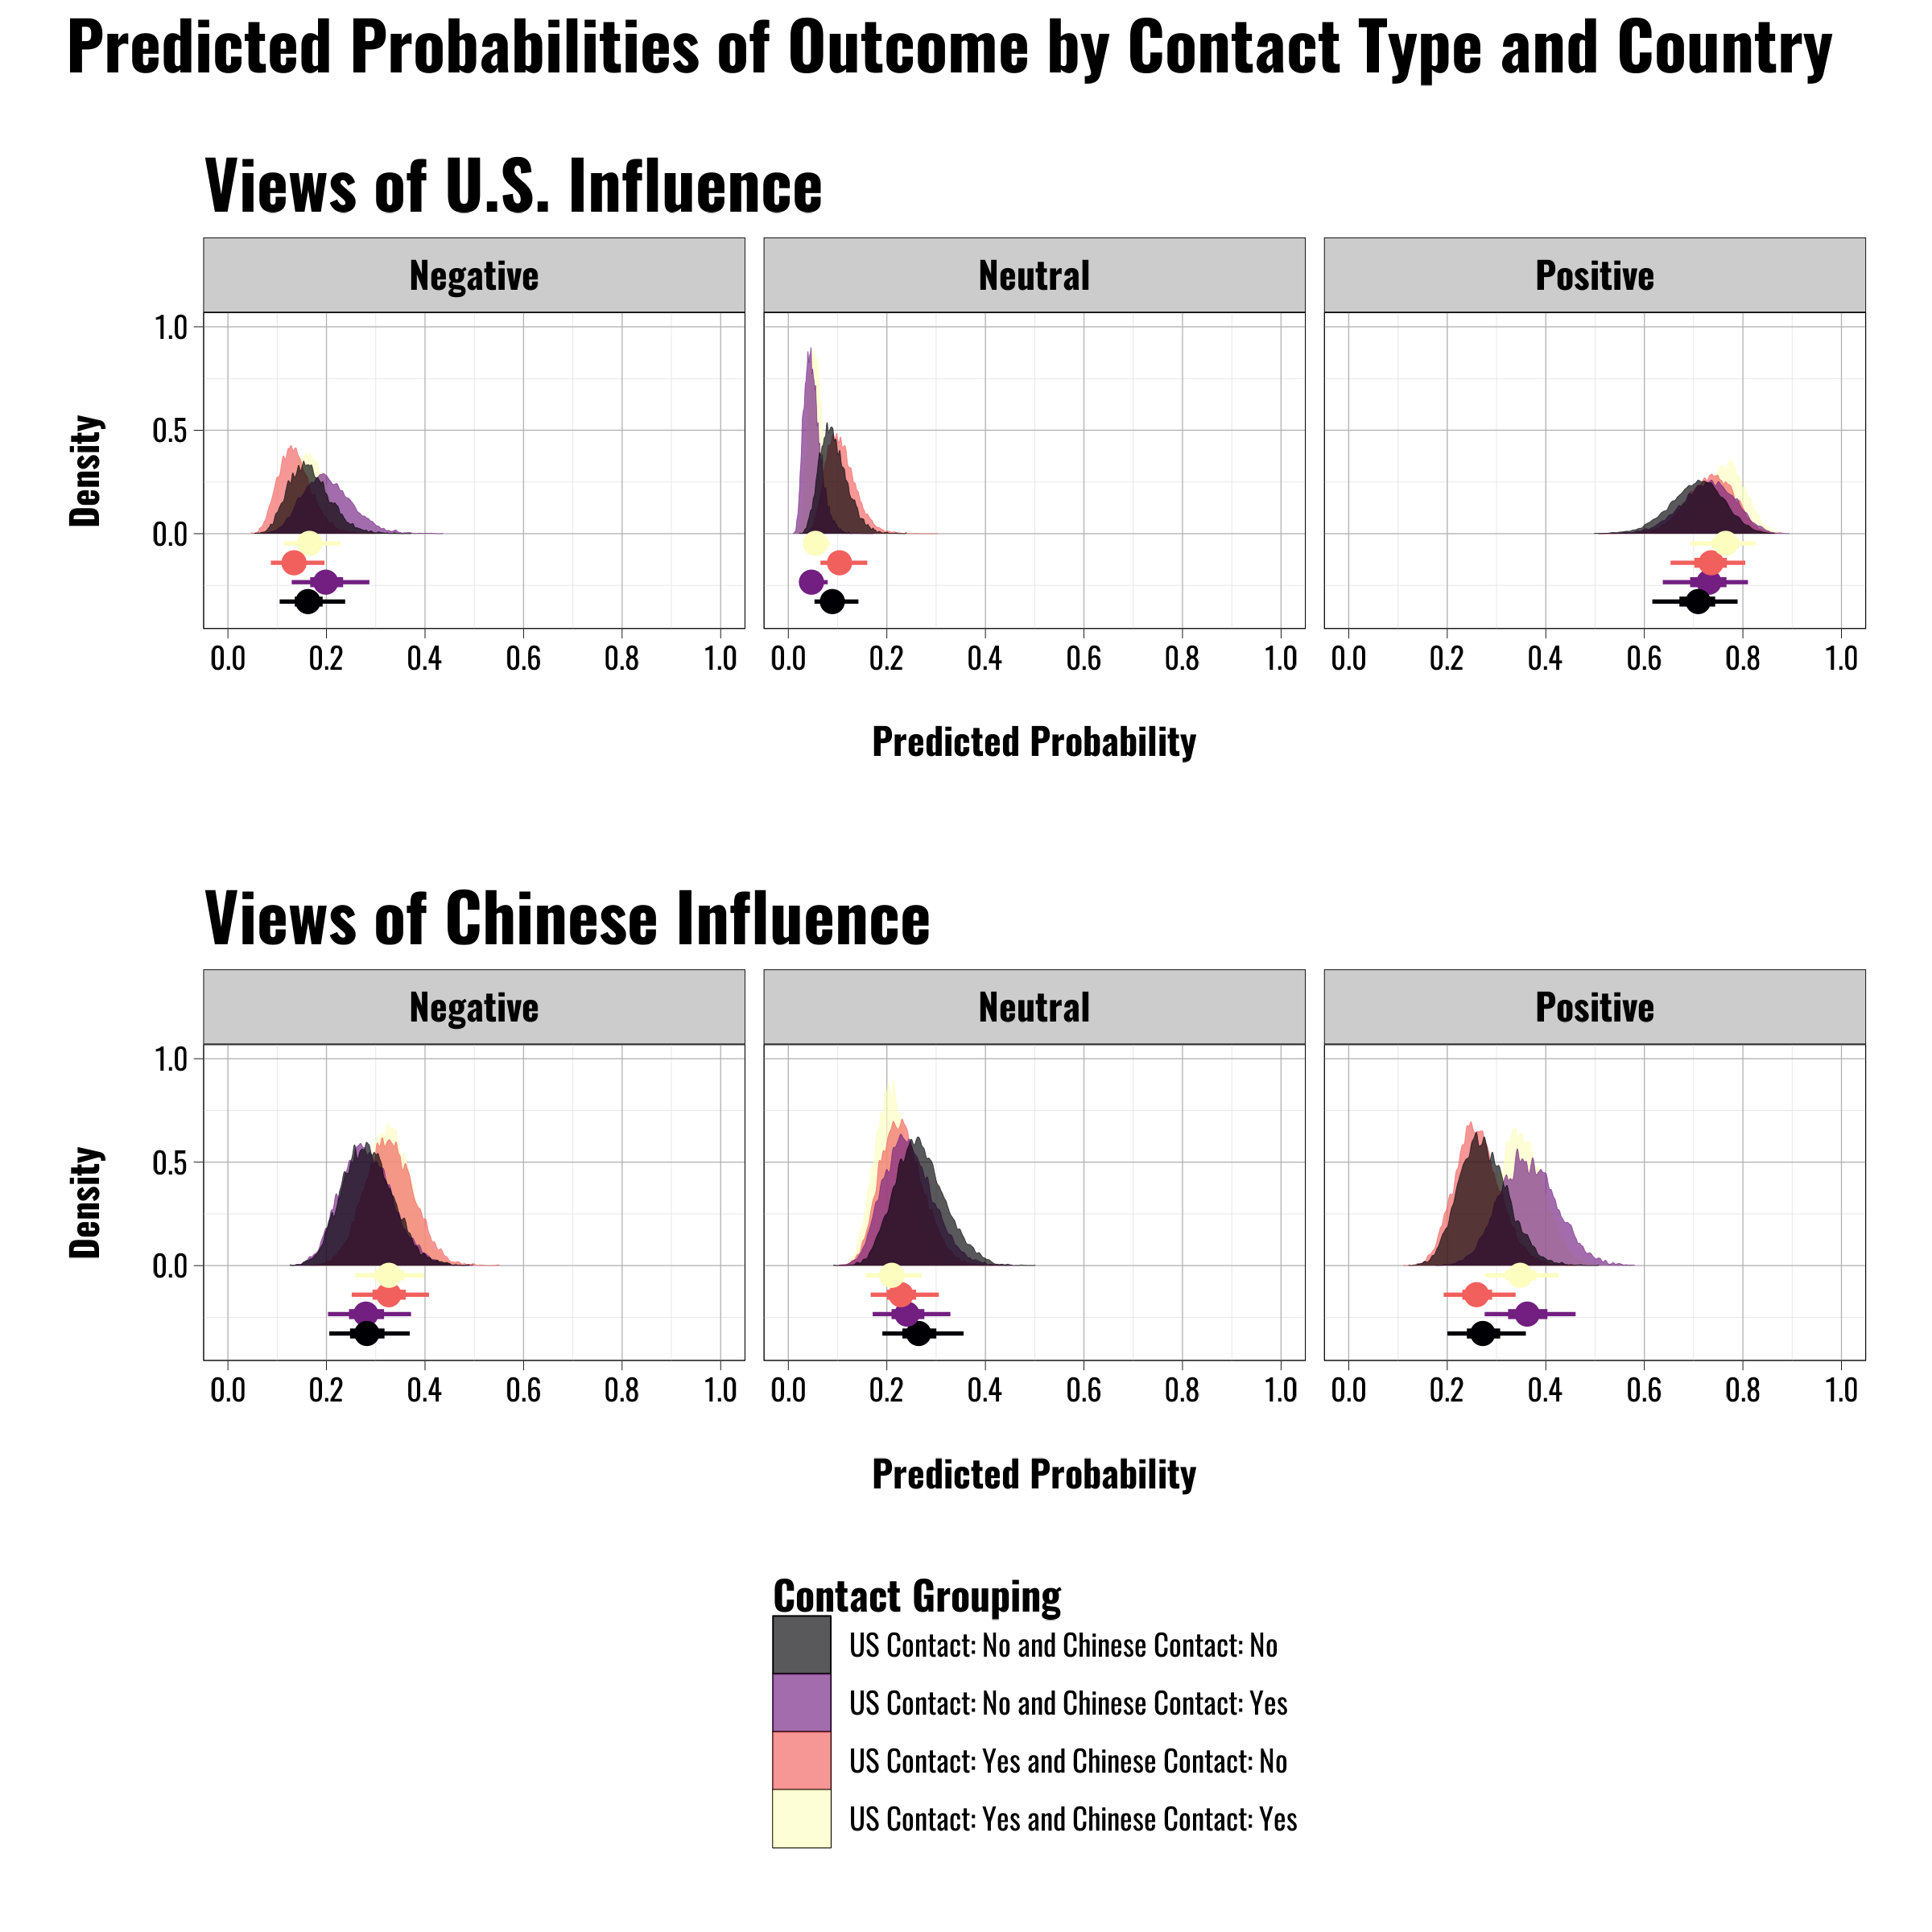
\includegraphics{../../Figures/Kenya-ISA/figure-predicted-probabilities.png}}
		\caption{Multinomial logit coefficient plot for primary variables of interest. \label{pp}}
	\end{center}
\end{figure}

Figure \ref{pp} contains the estimations of our fully specified model when we condition the view of each country's influence on whether they have had contact with individuals from either the United States or China. While there is overlap in these posterior estimations, there is substantive movement in a few cases. In the U.S. influence models, the baseline level of support is very high, making deviation on any graph more difficult as there is less room to go higher on positive and negative views. However, those with U.S. contact are less likely to have negative views and those with Chinese contact are more likely to have negative views. Likewise, those with Chinese contact are less likely to view the United States negatively.

In the Chinese influence models, we see similar movements as well. Those with U.S. contact, but not Chinese contact, are more likely to report negative views of Chinese influence. Those with either contact are less likely to have neutral views on the subject. Finally, Kenyans with exclusively Chinese contact are far more likely to have positive views of Chinese influence. In all six estimations, this last shift is the largest.

	\section*{Conclusion}


\newpage


\bibliography{Kenya}



\end{document}